\section{Méthode}

\subsection{Dataset}

Nous utilisons le dataset fournit pour la tâche 3 de l’édition 2009 de DEFT.
Il s'agit d'un corpus multilingue de débats parlementaires européens. Chaque intervention
parlementaire est classée en fonction du parti \footnote {ELDR, PPE-DE, PSE, GUE-NGL et Verts-ALE}
du locuteur et présente dans le corpus dans 3 langues : anglais, français et italien.\\
Au moment de faire des statistiques descriptives, nous nous sommes rendus comptes 
que le corpus présentait des doublons, et ce majoritairement dans la partition test.
\begin{figure}[ht]
    \centering
    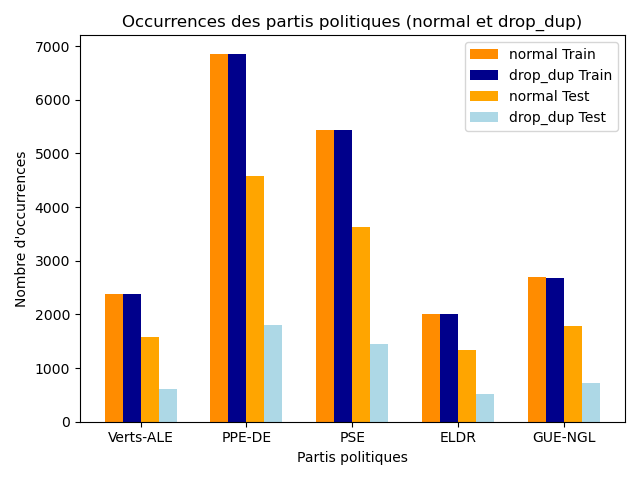
\includegraphics[width=\columnwidth]{../stats/occurences_orig_vs_drop_dup_par_cat.png}
    \caption{Nombre d'interventions par parti par partition test/train, dans le corpus original et dans la version sans doublons}
    \label{fig:barplot_dataset}
\end{figure}

Après suppression des doublons, la partition prévu (40/60) est changée : elle est 
maintenant de 20/80\footnote{ 0.79 pour le train et 0.21 pour le test}.
Nous avons envisagé de refaire le partitionnement pour réimplémenter le partitionnement 
prévu, mais avons renoncé pour deux raisons : 
refaire le partitionnement nous éloigne, encore, du corpus initialement prévu, et les 
résultats de quelques modèles sur un corpus repartitionné étaient proches des résultats 
sur cette partition 80/20.
Par ailleurs, la répartition des classes est déséquilibrée : les classes PPE-DE et PSE forment à elles deux 63,5 \% du corpus. Ceci devra être 
pris en compte dans le prétraitement.\footnote{la figure correspond au train, mais la répartition est sensiblement la même dans le test}

\begin{table}[ht]
    \centering
\begin{tabular}{|l|l|l|}
\hline
Statistique & Test & train 3 \\ \hline
Moyenne & 3871.4 & 1021.2 \\ \hline
STD & 2149.1 & 569.7 \\ \hline
Min & 2005.0 & 525.0 \\ \hline
1er quartile & 2376.0 & 615.0 \\ \hline
Médiane & 2687.0 & 715.0\\ \hline
3eme quartile & 5431.0 & 1448.0\\ \hline
Max & 6858.0 & 1803.0\\ \hline
\end{tabular}
\caption{Nombres d'intervention par parti par partition}
\label{tab:stats_dataset}
\end{table}

\begin{figure}[ht]
    \centering
    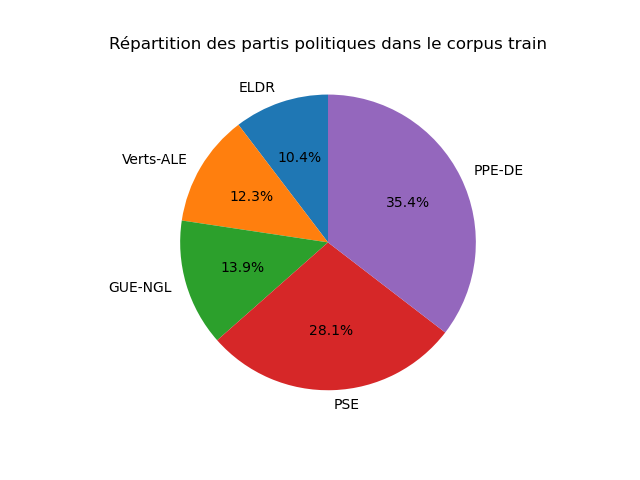
\includegraphics[width=\columnwidth]{../stats/occurences_par_partis_train_camember.png}
    \caption{Répartition des interventions par parti dans la partition train sans doublons}
    \label{fig:camember_dataset}
\end{figure}
\subsection{Prétraitements}
Le texte des interventions a été soumis à un prétraitement simple :\\
\indent(1) Suppresion de la ponctuation\\
\indent(2) Unification de la casse en minuscules\\
\indent(3) Tokenisation\footnote {Une lemmatisation avec la bibliothèque SpaCy a été envisagée,
mais ce corpus multilingue aurait nécessité le chargement de 3 modèles linguistiques
différents et ralongé d'autant le temps de traitement}
\\
Pour résoudre le problème de déséquilibre des classes, nous avons opté pour le \textit{downsampling} afin d'obtenir des classes relativement équilibrées,
en utilisant la fonction \textit{resample} de la bibliothèque Sckit-learn.

\begin{table}[ht]
    \centering
\begin{tabular}{|l|l|l|}
\hline
Parti & Test & train 3 \\ \hline
Moyenne & 3871.4 & 1021.2 \\ \hline
STD & 2149.1 & 569.7 \\ \hline
Min & 2005.0 & 525.0 \\ \hline
1er quartile & 2376.0 & 615.0 \\ \hline
Médiane & 2687.0 & 715.0\\ \hline
3eme quartile & 5431.0 & 1448.0\\ \hline
Max & 6858.0 & 1803.0\\ \hline
\end{tabular}
\caption{Nombres d'intervention par parti par partition}
\label{tab:stats_dataset}
\end{table}


\subsection{Les différents embeddings}